We performed an end-to-end evaluation of our prototype in a cluster with 5 test nodes.
The cluster is connected to a 5-shelves PanFS storage system
with 5 metadata nodes and 50 storage nodes.
Since each test node has 64 cores and a 40GE NIC, they are able to
to saturate the data bandwidth of our PanFS storage cluster.
Because of some technique difficulties,
we did not run our \sys server process inside the metadata node.
Instead, we co-locate our \sys server processes
with client processes in the test nodes.
Each test node runs a \sys server that is assigned to a metadata node
as explained in Section \ref{design.integration}.
The system of layering \sys on top of PanFS is called \psys through
this evaluation section.
We ran a series of HPC benchmarks (used by parallel file system vendors and users)
to test metadata path and data path separately,
including the open source \textit{mdtest} synthetic benchmark \cite{mdtest}
and File System Test Suite checkpoint benchmark from LANL \cite{mpiio}.

\textbf{Metadata intensive workloads -- }
We used the synthetic mdtest benchmark \cite{mdtest}
to generate a three-phase workload:
The first phase is to create 5 million
zero-files in a single shared directory \cite{ceph:weil06, GIGA11};
the second phase is to perform $stat()$ on random files in the directory;
the third phase is to delete all the files in the directory in a random order.
Each phase involves multiple clients to issue the operations concurrently.

If we directly use the above workload to directly compare our layered system
against the original PanFS, it would not be fair enough.
This is because a single directory can only utilize the hardware resource
of one metadata manager in PanFS,
and PanFS also limits a single directory to 1 million files.
Therefore we chose to compare native PanFS creating 1 million files
in 5 different directories owned by 5 different metadata managers.
The total number of clients used for testing the two systems
are kept the same.

\begin{figure}[t]  %%%%%%%%%%%%%%%%%%%%%%%
\centerline{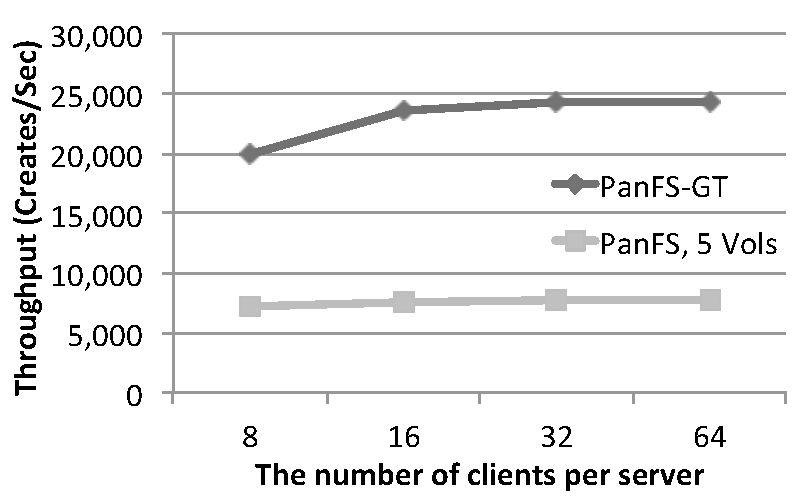
\includegraphics[scale=0.7]{./figs/zero_file_creation_on_panfs}}
\vspace{10pt}
\caption{\normalsize
\textit{Average throughput during creating five million zero-length files
in one empty directory with different number of clients per test node.
Running 32 and more clients per test node is able to saturate \psys
and original PanFS}
}
\vspace{10pt}
\hrule
\label{graph:creation_clients}
\end{figure}       %%%%%%%%%%%%%%%%%%%%%%%

\begin{figure}[t]  %%%%%%%%%%%%%%%%%%%%%%%
\centerline{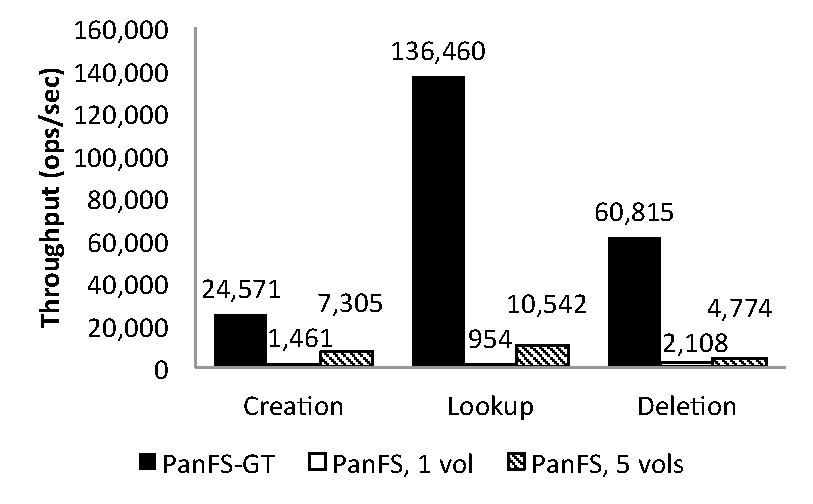
\includegraphics[scale=0.7]{./figs/mdtest}}
\vspace{10pt}
\caption{\normalsize
\textit{mdtest:
The average aggregated throughput of different operations in mdtest
when generating 5 million zero-length files in a single shared directory.
Since PanFS has a hard limit to allow only create 1 million entries
in one directory, the bar showing PanFS with 1 volume only gives
the average throughput for the case of creating 1 million entries.
}
}
\vspace{10pt}
\hrule
\label{graph:mdtest_ops}
\end{figure}       %%%%%%%%%%%%%%%%%%%%%%%


Figure \ref{graph:creation_clients} shows the aggregated througphut during
the first phase. We varies the nubmer of clients running in each test node
to find the right number that can saturate both systems.
Both systems achieve the highest aggregated throughput when the number
of clients per node is 32 or more. In all the experiments shown later,
we present the results with 32 clients per test node if without explanation.
For all cases, \psys is approximately 3.5 times faster than the native PanFS
using 5 volumes. The aggregated throughput with 32 clients per server
achieves about 24,571 creation per second.

Figure \ref{graph:mdtest_ops} shows the aggregated througphut of
different operations during three phases in mdtest.
Besides \psys and PanFS using 5 volumes, it also shows
the aggregated throughput of creating 1 million files in one volume of PanFS.
For $lookup$ and $deletion$ workloads,
\psys gains more advantages over original PanFS,
and achieves about 10 to 15 times speed up.
Fast lookup is due to the memory indexing and Bloom filters in \ldb.
For deletion of a key, \ldb essentially just inserts the key and a deletion mark
into its memtable, and delays the actual deletion in later compaction processes.


\textbf{Small file workloads -- }
We also use mdtest benchmark to generate files with small size data to evaluate
the effectiveness of embedding file content with the metadata inside \tfs.
Similar to the previous test,
mdtest benchmark creates 5 million files in a single directory
but with file data of two different sizes: 4KB and 16 KB.
4KB is the median file size for many desktop workloads \cite{Bill11},
and 16KB is the median file size for some large storage clusters using PanFS \cite{brent13}.
The threshold $T$ for our prototype is set to 64KB, so all these files
are stored in \tfs instance.

%compaction and CPU usage
Figure \ref{graph:smallfiles} shows the aggregated throughput during the test,
which is aggregated from all clients. For 4KB file size,
\psys is about $2.5\times$ faster than original PanFS.
However, \psys is about $35\%$ slower than PanFS for 16KB file size.
We found that embedding 16KB file makes the key-value pair significanly larger,
and causes higher write amplification during compaction process in \ldb,
since \ldb tries to merge sort both file data and metadata.
Additionally, \ldb will firstly write the inserted key-value pairs
to the transaction log, and then (during a compaction) to the SSTable.
With larger key-value pairs, LevelDB's per-operation efficiency is
slowed down by the cost of extra copies of large values.
This suggests that the threshold $T$ for embedding file size should not be
greater than 16 KB. For larger embedding file size,
we might sacrafice the read performance to maintain its fast insertion rate
by using column-based approach which stores metadata and small file separately.
Such investigation is left for future works.

\begin{figure}[t]  %%%%%%%%%%%%%%%%%%%%%%%
\centerline{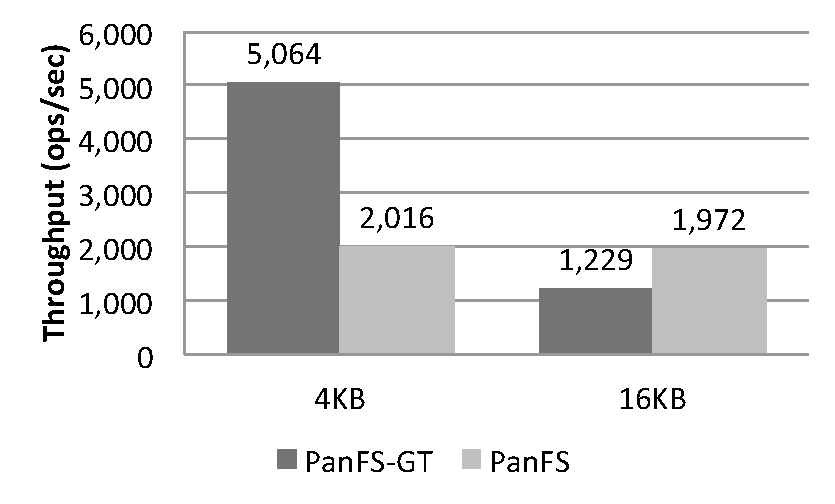
\includegraphics[scale=0.7]{./figs/small_file_creates}}
\vspace{10pt}
\caption{\normalsize
\textit{Average aggregated throughput during creating 5 million small files
with different sizes in one shared directory}
}
\vspace{10pt}
\hrule
\label{graph:smallfiles}
\end{figure}       %%%%%%%%%%%%%%%%%%%%%%%


%Library version not FUSE
%Clean cache

\textbf{Data intensive workloads -- }
The LANL filesystem checkpoint benchmark can
generate many types for HPC checkpoint I/O patterns.
For our test purposes, we configured the benchmark to generate
a concurrent N-N checkpoint write and read workload.

All checkpoint file I/O is performed by a set of processes
that synchronize with each other using MPI barriers.
At the begining, each process opens a freshly created checkpoint file
for writing and then waits at a barrier until all processes are ready to write.
Once all processes are ready, each processes starts
concurrently writing the checkpoint data to its own file,
until it has written the specified number of bytes.
It then waits barrier for all the other processes to finish writing,
and finally syncs its data to the file system and closes the file.
Before starting the read phase we terminate all processes
accessing these checkpoint files so that
we can unmount the filesystem in order to ensure that
all freshly written data has been flushed out from all the nodes' memory
to prevent caching from unfairly biasing our read performance.
After the filesystem has been mounted and restarted,
the benchmark reads the checkpoint in the same way it was written,
however we shift, so each process will read
the file generated by another process.

In this test, we also vary the number of clients per test node
from 8 to 64 clients. The clients in each node will generate
640GB checkpoint data in total to the underlying file system,
no mater what number of clients each node has.
The size of data buffer for each file system call is set to be 16KB.
For \psys, the checkpoint files generated in the test will be
first stored in \tfs, and then migrated to the underlying PanFS.

Figure \ref{graph:checkpoint_write} and \ref{graph:checkpoint_read}
show the average throughput during the write phase and read phase
in the N-N checkpoint workload respectively. We can see \psys
performs comparably with the native PanFS.
For read checkpoint worload, the largest performance loss is less than $10\%$.
And \psys is even faster in write checkpoint phase.
The embedding of small files do not affect the data transfers
of large files.

\begin{figure}[t]  %%%%%%%%%%%%%%%%%%%%%%%
\centerline{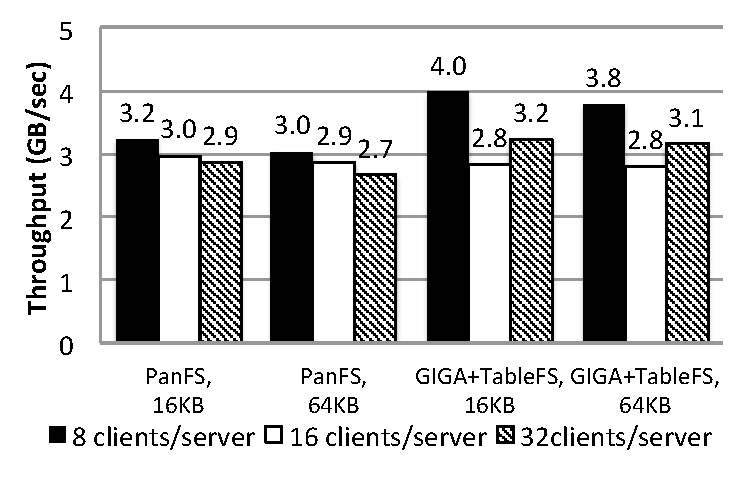
\includegraphics[scale=0.7]{./figs/checkpointing_write}}
\vspace{10pt}
\caption{\normalsize
\textit{
The aggregated write throughput in N-N check-pointing workload.
Each volume receives 640 GB data.
}
}
\vspace{10pt}
\hrule
\label{graph:checkpoint_write}
\end{figure}       %%%%%%%%%%%%%%%%%%%%%%%

\begin{figure}[t]  %%%%%%%%%%%%%%%%%%%%%%%
\centerline{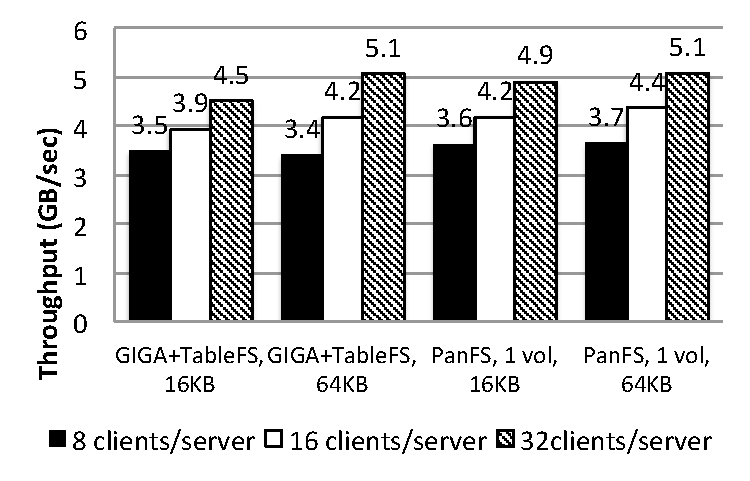
\includegraphics[scale=0.7]{./figs/checkpointing_read}}
\vspace{10pt}
\caption{\normalsize
\textit{
The aggregated read throughput in N-N check-pointing workload.
}
}
\vspace{10pt}
\hrule
\label{graph:checkpoint_read}
\end{figure}       %%%%%%%%%%%%%%%%%%%%%%%

